\documentclass[10pt,aspectratio=169]{beamer}

% Font encoding and font packages
\usepackage[T1]{fontenc}
\usepackage{lmodern}

% Theme and styling
\usetheme{Madrid}
\usecolortheme{default}
\setbeamertemplate{navigation symbols}{}
\setbeamertemplate{footline}[frame number]

% Increase title  \item \emph{Imitation learning:} compute \textbf{Oracle RRI} by exhaustive "add-and-reconstruct" for 120 query views per object; train VIN to imitate without rendering.
  \item Reformulate as \textbf{ordinal classification} into $K{=}15$ bins with a ranking-aware CORAL loss and \textbf{stage-wise} z-score normalization.
\end{itemize}
\end{frame}

\section{Design Considerations}

\begin{frame}{Hulls/OBBs First?} font sizes
\setbeamerfont{title}{size=\Huge,series=\bfseries}
\setbeamerfont{author}{size=\Large}
\setbeamerfont{institute}{size=\large}
\setbeamerfont{date}{size=\large}

% Packages
\usepackage{amsmath}
\usepackage{amssymb}
\usepackage{pifont}
\usepackage{xcolor}
\usepackage{tikz}
\usepackage{subcaption}
\usepackage{graphicx}
% Bibliography support - use numbers mode for ieeetr style
\usepackage[numbers]{natbib}
% \usepackage{algorithm}
% \usepackage{algorithmicx}
% \usepackage{algpseudocode}
\usepackage{mathtools}
\usepackage{bm}

\definecolor{mygreen}{rgb}{0,0.6,0}
\definecolor{myred}{rgb}{0.8,0,0}
\newcommand{\greenoplus}{\textcolor{mygreen}{\( \oplus \)}}
\newcommand{\redominus}{\textcolor{myred}{\( \ominus \)}}

% Custom commands
\newcommand{\R}{\mathbb{R}}

% Title information
\title{Interactive Next-Best-View (NBV) for Streaming Reconstruction}
\author{Jan Duchscherer}
\institute{%
  Hauptseminar \\[0.5ex]
  Department of Computer Science and Mathematics\\[1ex]
  Lecturer: Prof.\ Dr.\ Markus Friedrich
}
\date{\today}
\titlegraphic{%
  \vspace{1em}%
  \hfill
\includegraphics[height=1.2cm]{../figures/hm-logo.pdf}%
}

\begin{document}

% Title slide
\begin{frame}[plain]
  \titlepage
\end{frame}

% Outline slide
\begin{frame}{Outline}
\tableofcontents
\end{frame}

\section{Active Reconstruction: Domain Challenges}

\begin{frame}{Problem Landscape}
\textbf{Objective:} Maximize 3D \emph{quality} under budgets (frames, time, path length) while staying interactive.
\begin{itemize}
  \item Decision variables: next pose(s) or short \textbf{pose sequence}; reachability + motion constraints.
  \item Trade-offs: quality gain vs. capture cost; exploration vs. refinement; coverage vs. fidelity.
  \item Streaming constraints: on-device \textbf{latency}, memory; human-in-the-loop guidance.
  \item Score choice: coverage proxies vs. \textbf{RRI} (relative error drop) as NBV fitness.
\end{itemize}
\end{frame}

\begin{frame}{Failure Modes, Constraints, and Evaluation}
\textbf{Common pitfalls}
\begin{itemize}
  \item Occlusions, thin/reflective/textureless surfaces; rolling-shutter and depth noise.
  \item Pose drift, poor loop-closure; moving objects and exposure changes.
  \item Combinatorial candidate sampling; physical feasibility and safety margins.
\end{itemize}
\textbf{System constraints}
\begin{itemize}
  \item Low-latency scoring in \textbf{streaming} capture; robust pose estimation; AR legibility.
  \item Source of semantics: \textbf{OBBs/hulls}, SceneScript primitives, or VLM-based importance.
\end{itemize}
\textbf{Evaluation signals}
\begin{itemize}
  \item Quality: Chamfer/F-score; \textbf{RRI} per step; completeness vs. accuracy.
  \item Efficiency: frames, path length, runtime/step; user interventions.
  \item Coverage baselines: AUC-coverage and novelty/empty-pixel reduction.
\end{itemize}
\end{frame}

\section{Goal \& Seminar MVP}

\begin{frame}{Aim \& Relative Reconstruction Improvement (RRI)}
\begin{block}{Project Aim}
Interactive, \textbf{streaming} NBV guidance that proposes next camera poses for optimal quality gains and reports a per-view \textbf{RRI} score.
\end{block}

\textbf{RRI definition (conceptual):}
\begin{equation*}
\mathrm{RRI}(q)=\frac{E(R_{\text{base}})-E(R_{\text{base}}\cup q)}{E(R_{\text{base}})} \quad
\text{with } E(\cdot) \text{ a reconstruction error (e.g., Chamfer).}
\end{equation*}

\textbf{Seminar MVP:}
\begin{itemize}
  \item Streaming loop: maintain live recon; evaluate sampled candidates; select max-RRI; iterate.
  \item Baseline: cheap \textit{coverage} score (holes/empty pixels).
  \item \textit{Semantic value}: prioritize entities/regions that matter to the user/task.
\end{itemize}
\end{frame}

\begin{frame}{Scoring Signals \& Streaming Loop}
\textbf{Scoring signals (concise):}
\begin{itemize}
  \item \textbf{Coverage \/ novelty:} unseen area, empty-pixel ratio (inside\/outside hull).
  \item \textbf{Geometry \& uncertainty:} normal variance, view angle, baseline, depth\/TSDF variance.
  \item \textbf{Entity-aware (optional):} per-object coverage and facet visibility (OBBs\/primitives).
\end{itemize}

\textbf{Streaming NBV loop:}
\begin{enumerate}
  \item Update reconstruction from latest frames.
  \item Sample candidate poses in reachable space.
  \item Compute features (\textit{coverage} + geometry + entity stats).
  \item Predict RRI; suggest top-$k$ views; accept human nudge.
\end{enumerate}
\end{frame}

\section{Key Papers (1 slide each)}

\subsection{SceneScript}
\begin{frame}{SceneScript --- Parametric Scene Programs}
\textbf{Key contributions}~\cite{SceneScript-avetisyan2024}
\begin{itemize}
  \item Structured \textbf{scene program} with parameterized primitives (layout + geometry).
  \item Autoregressive decoder enables \textbf{editability} and compositional reasoning.
  \item Differentiable projection losses align program with sensor data.
\end{itemize}
\textbf{Method features}
\begin{itemize}
  \item Point-cloud encoder $\rightarrow$ program tokens (walls, doors, windows, etc.).
  \item Grammar of primitives; MR-friendly updates; explicit entities.
  \item Mostly \textbf{architectural} categories (limited object vocabulary).
\end{itemize}
\textbf{Relevance to NBV}
\begin{itemize}
  \item Provides \textbf{entities/OBBs} for per-entity coverage, uncertainty, and semantic value.
  \item Natural fit for entity-aware guidance and per-facet view planning.
\end{itemize}
\end{frame}

\subsection{HITL Infilling}
\begin{frame}{HITL Infilling for SceneScript}
\textbf{Key contributions}~\cite{HITL-SceneScript-xie2025}
\begin{itemize}
  \item \textbf{Human-in-the-loop} local corrections via \emph{Infill}, \emph{Add}, and \emph{Delete}.
  \item Locality-constrained edits; mixed-reality interaction at interactive rates.
\end{itemize}
\textbf{Method features}
\begin{itemize}
  \item Masked \textbf{infilling} over the scene program with point-guided repair.
  \item One-click selection of a region; model proposes consistent completion.
\end{itemize}
\textbf{Relevance to NBV}
\begin{itemize}
  \item UX template for \textbf{interactive guidance}: user biases which entities/regions to favor.
  \item On-the-fly \textbf{entity corrections} (hulls/boxes) feeding the scoring pipeline.
\end{itemize}
\end{frame}

\subsection{GenNBV}
\begin{frame}{GenNBV --- RL for Next-Best-View}
\textbf{Key contributions}~\cite{GenNBV-chen2024}
\begin{itemize}
  \item Generalizable NBV policy in \textbf{5-DoF} continuous action (3D position + yaw/pitch; roll fixed).
  \item Multi-source \textbf{state}: probabilistic 3D occupancy grid + semantic embedding + action history.
  \item Coverage-oriented reward (AUC of coverage) with penalties (collisions, excessive keyframes).
\end{itemize}
\textbf{Method features}
\begin{itemize}
  \item Actor outputs a Gaussian over 5-DoF; trained with PPO.
  \item Depth back-projection distinguishes unscanned vs. free space; semantics from CNN over RGB.
  \item Encodes recent actions to stabilize exploration vs. exploitation.
\end{itemize}
\textbf{Relevance to NBV}
\begin{itemize}
  \item Blueprint for \textbf{coverage/uncertainty} features and safe handheld trajectories.
  \item Baseline/ablation target vs. learned improvement prediction (VIN-NBV).
\end{itemize}
\end{frame}

% Start of slides on VIN-NBV
\subsection{VIN-NBV}
\begin{frame}{VIN-NBV --- Motivation and Key Idea}
\textbf{Claimed limitations of prior methods}~\cite{VIN-NBV-frahm2025}
\begin{itemize}
  \item Coverage maximization is an imperfect \textbf{proxy} for quality (fails with occlusions and fine details).
  \item RL-based policies optimize coverage/safety, not reconstruction \textbf{quality}; need many interactions.
  \item Assumptions about prior scene knowledge hurt generalization.
\end{itemize}

\vspace{1em}
\textbf{Key idea}\;\textemdash\;\emph{predict reconstruction \textbf{quality} gain directly.}

\begin{equation*}
\mathrm{RRI}(q)=\frac{CD(R_{\text{base}},R_{GT})-CD(R_{\text{base}}\cup q,\,R_{GT})}{CD(R_{\text{base}},R_{GT})}
\end{equation*}

\vspace{0.5em}
\textbf{NBV objective}
\begin{equation*}
C^{*}_{nbv}=\arg\max_{C_{nbv}} \; \frac{CD(R_{\text{base}},R_{GT})-CD(R_{\text{final}},R_{GT})}{CD(R_{\text{base}},R_{GT})}
\end{equation*}
\end{frame}

\begin{frame}{VIN-NBV --- System Overview}
\begin{figure}
  \centering
  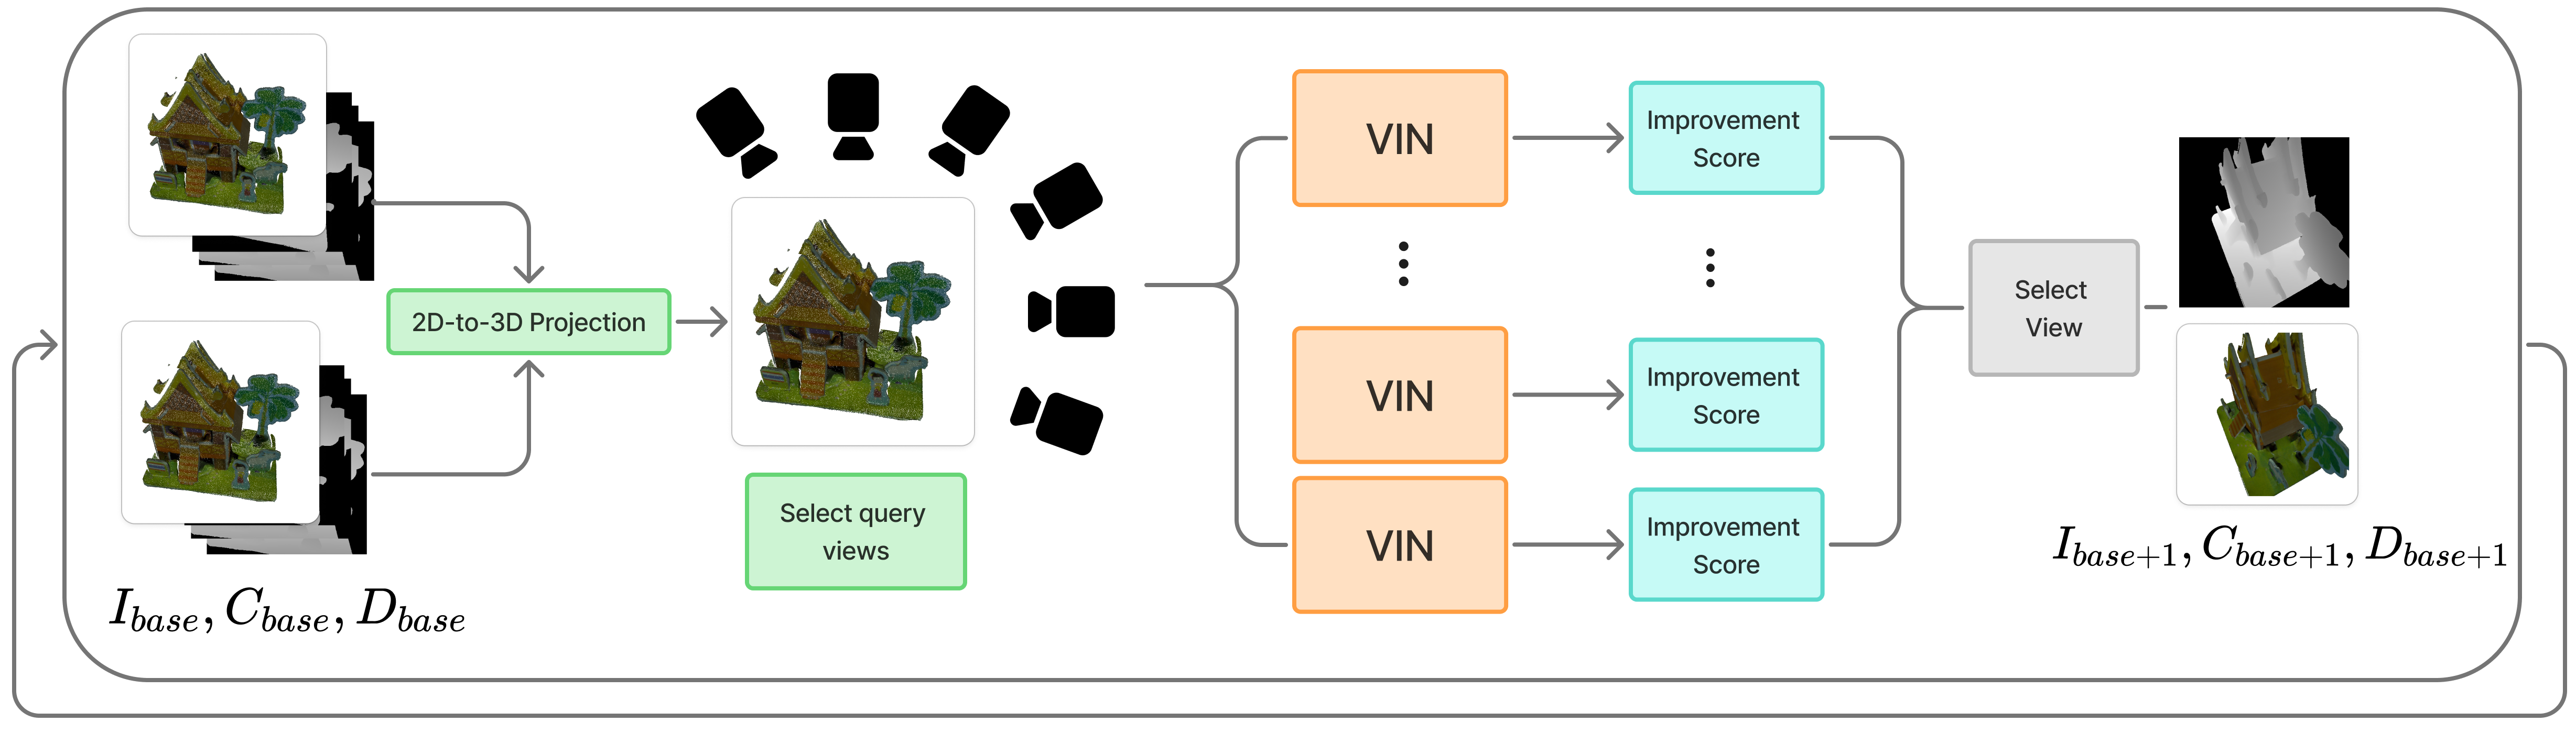
\includegraphics[width=0.95\textwidth]{../../literature/tex-src/VIN-NBV/Figures/VIN-NBV_diagram.png}
  \caption{VIN-NBV pipeline: from base views to candidate evaluation and view selection.}
\end{figure}
\end{frame}

\begin{frame}{VIN-NBV --- Architecture}
\begin{columns}[T]
\begin{column}{0.58\textwidth}
\textbf{Input:} Base RGB-D $I_{\text{base}}$, $C_{\text{base}}$, $D_{\text{base}}$; candidate view $q$

\vspace{0.5em}
\textbf{Output:} \(\widehat{\mathrm{RRI}}(q)\) score for greedy selection

\vspace{0.5em}
\textbf{3D-aware features:}
\begin{itemize}
  \item Reconstruct $R_{\text{base}}$ with normals, visibility, depth variance
  \item Project to query: $F_g$, $F_e$, $F_{\text{empty}}$
  \item CNN encode: $\widehat{\mathrm{RRI}}(q)=M(V_{\text{view}}\oplus f_{\text{base}}\oplus f_{\text{pose}})$
\end{itemize}

\vspace{0.5em}
\textbf{Training:} Oracle RRI (120 views/object) $\rightarrow$ ordinal classification (15 bins, CORAL loss)
\end{column}
\begin{column}{0.40\textwidth}
\vspace{-1em}
\begin{figure}
  \centering
  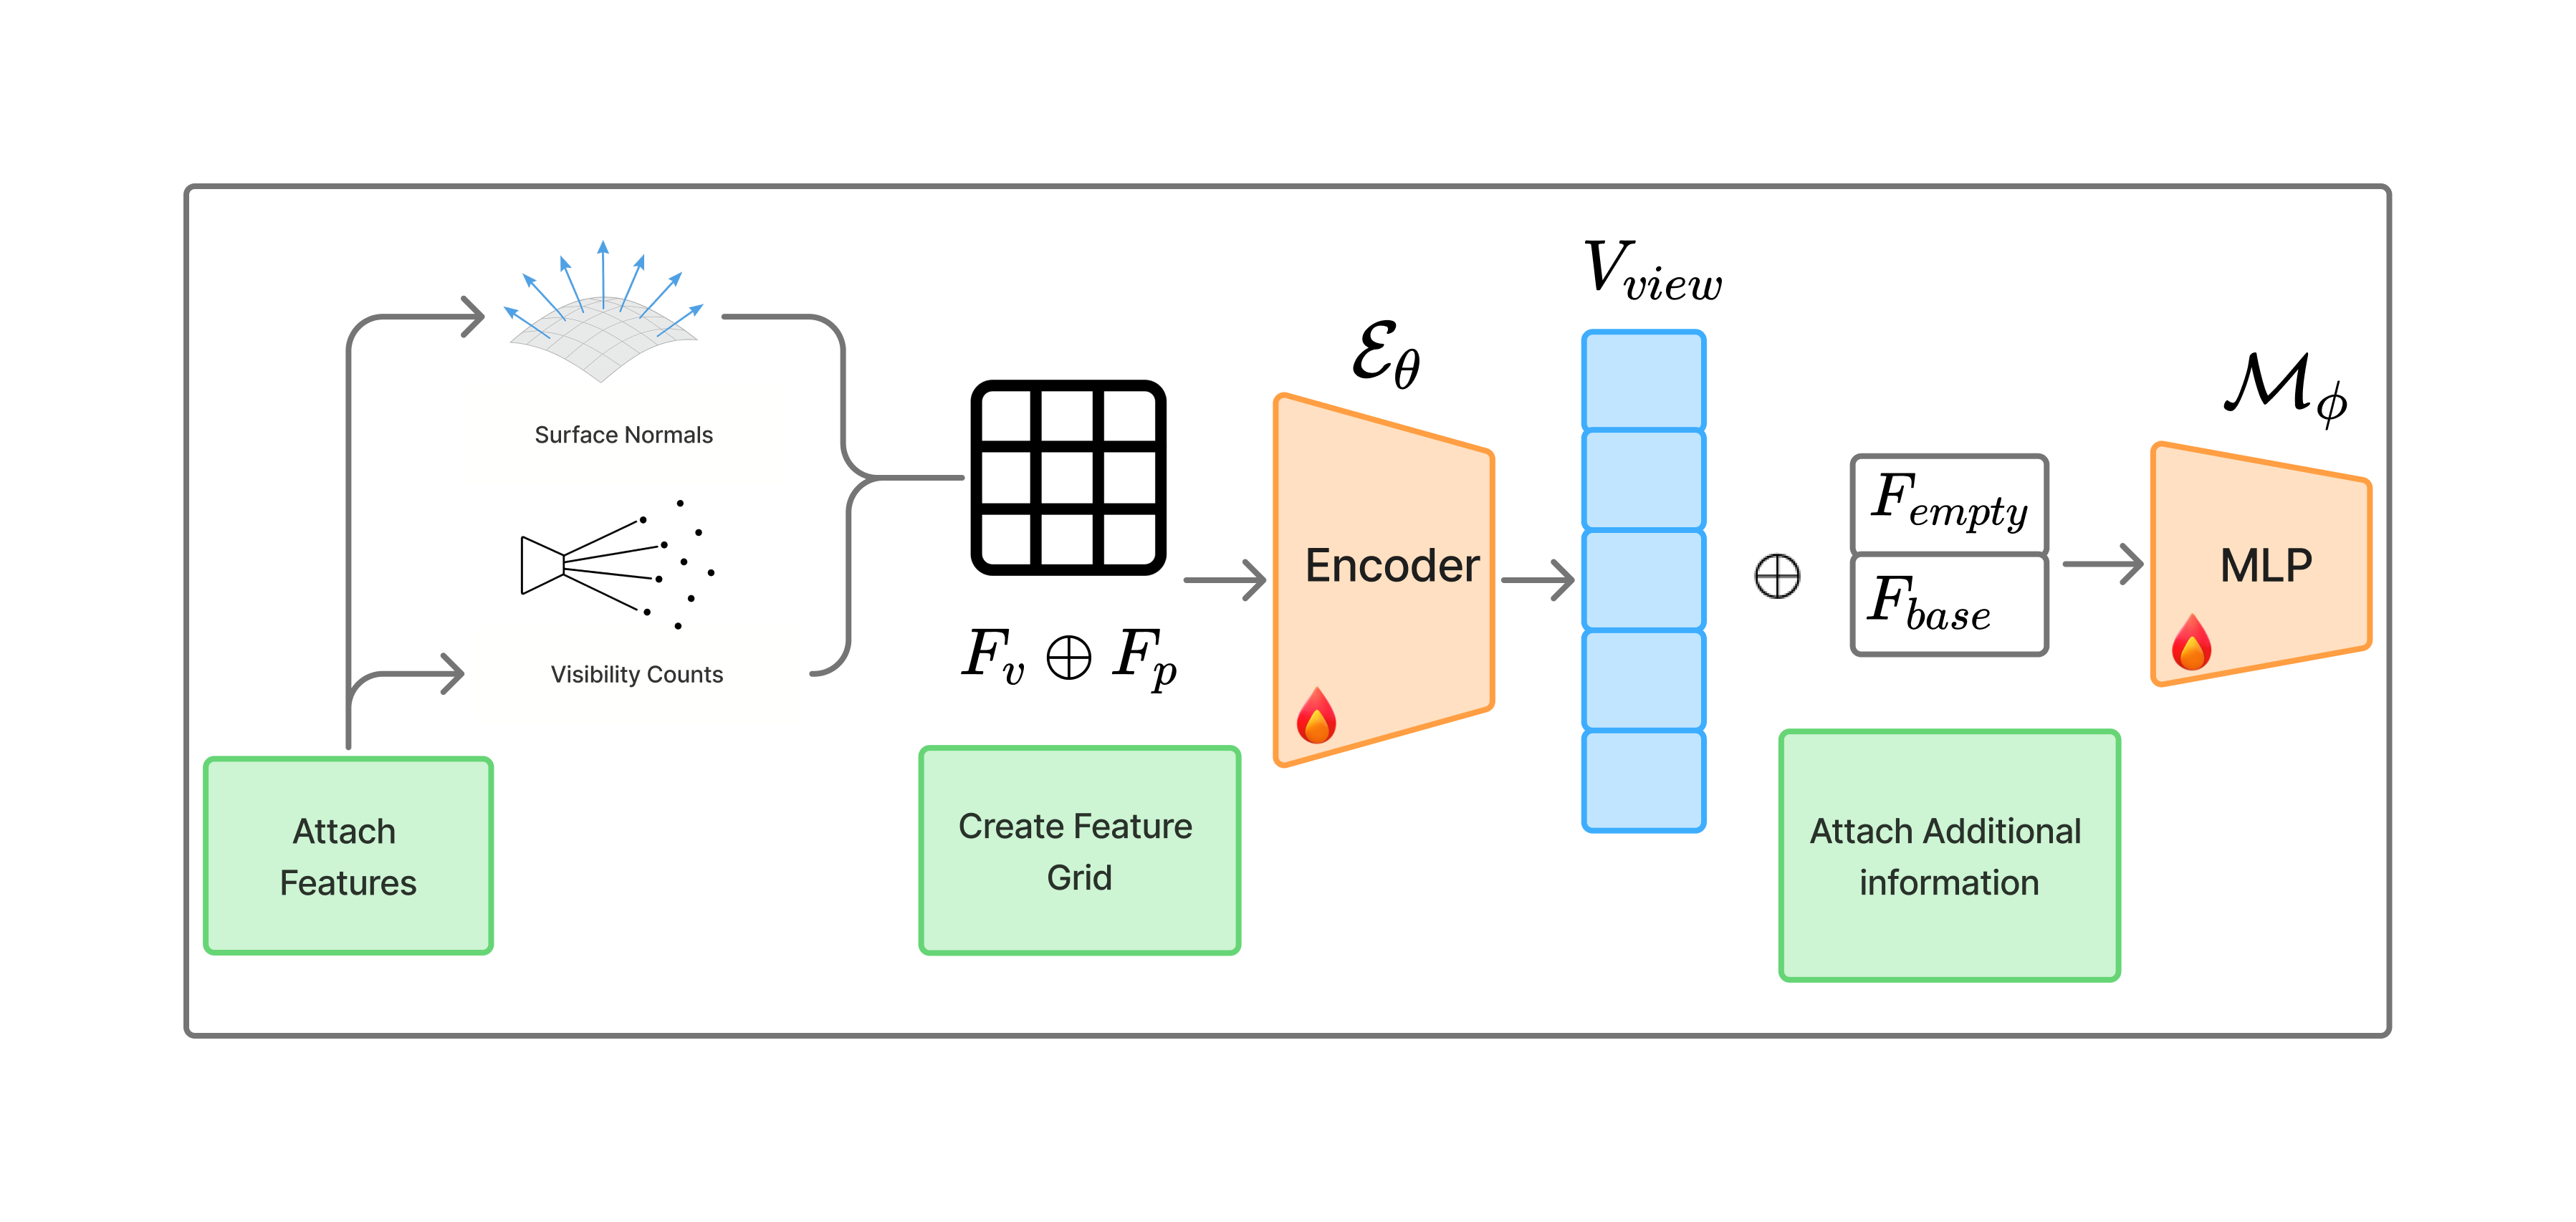
\includegraphics[width=\textwidth]{../../literature/tex-src/VIN-NBV/Figures/VIN_arch.png}
\end{figure}
\end{column}
\end{columns}
\end{frame}

\section{Design Considerations}
\begin{itemize}
  \item Reconstruct a point cloud $R_{\text{base}}$; enrich each point with \emph{surface normals}, \emph{visibility count}, and \emph{depth variance}.
  \item Project into the query image to form per-pixel features: geometric variance $F_g$, enriched features $F_e$, and \textbf{empty-pixel} maps $F_{\text{empty}}$ (inside/outside hull).
  \item Encode with a CNN: $V_{\text{view}}=E_i(F_g, F_e, F_{\text{empty}})$; concatenate number of base views $f_{\text{base}}$ and pose cues; predict
  \(\widehat{\mathrm{RRI}}(q)=M\!\left(V_{\text{view}}\oplus f_{\text{base}}\oplus f_{\text{pose}}\right)\).
\end{itemize}
\textbf{Training}
\begin{itemize}
  \item \emph{Imitation learning:} compute \textbf{Oracle RRI} by exhaustive “add-and-reconstruct” for 120 query views per object; train VIN to imitate without rendering.
  \item Reformulate as \textbf{ordinal classification} into $K{=}15$ bins with a ranking-aware CORAL loss and \textbf{stage-wise} z-score normalization.
\end{itemize}

\begin{frame}{Hulls/OBBs First?}
\textbf{Pros} \greenoplus
\begin{itemize}
  \item Enables \textbf{per-entity} coverage/RRI and user-intent weighting.
  \item Aligns with SceneScript editability; simple \textbf{facet-level} view planning.
  \item Simplified problem: global scene to local entities; smaller state space.
\end{itemize}
\textbf{Cons} \redominus
\begin{itemize}
  \item Extra engineering (OBB estimation or SceneScript adaptation).
  \item May not beat strong \textbf{point-centric} RRI features in practice.
  \item Sources for OBBs: fast depth clustering; VLM-based OBBs (e.g., Gemini); or adapted SceneScript.
\end{itemize}
\textbf{Pragmatic plan}
\begin{itemize}
  \item Start with VIN-style \textbf{point-centric RRI}; add \textbf{entity layer} as a re-ranker.
  \item For seminar: quick OBB proxies (depth clustering) before full SceneScript retune.
\end{itemize}
\end{frame}

\begin{frame}{Seminar MVP \& Minimal Ablations}
\textbf{MVP pipeline}
\begin{enumerate}
  \item Live recon (RGB-D/MVS) $\rightarrow$ candidate sampling.
  \item Compute features (coverage+geometry+$\pm$OBB stats).
  \item Predict RRI; display top-$k$ views \& \textbf{RRI bars}; user can bias ranking.
\end{enumerate}
\textbf{Ablations (short runs)}
\begin{itemize}
  \item \textbf{RRI vs. Coverage} (same sampler); with/without \textbf{entity re-ranking}.
  \item Drop/add features: uncertainty grid, normal variance, view-angle terms.
\end{itemize}
\end{frame}

\begin{frame}{Additional Considerations from Notes}
\textbf{Entity-/semantics-aware scoring}
\begin{itemize}
  \item \textbf{Uncertainty per entity}: aggregate visibility/TSDF variance per primitive/OBB; emit as a token.
  \item \textbf{Proxy objects}: quick hulls/OBBs for semantically relevant items when full SceneScript is unavailable.
  \item \textbf{Semantic quality score}: per-entity or per-volume; combine geometric intricacy with task importance (VLM predictor candidate).
\end{itemize}
\textbf{Novelty/coverage signals}
\begin{itemize}
  \item Expected \textbf{novelty} \/ coverage gain beyond current hull; measure unseen facets/empty pixels.
  \item \textbf{Coverage proxies}: Gaussian Splatting or structure-from-silhouette for fast fidelity checks.
\end{itemize}
\textbf{Systems/UX}
\begin{itemize}
  \item Natural-language + AR guidance; user can bias entities/regions.
  \item Consider direct \textbf{pose-sequence} prediction (tokenized NBV trajectory) vs. per-view scoring.
  \item Evaluation with RealityScan/Polycam; watch \textbf{pose-estimation} reliability.
\end{itemize}
\end{frame}

\section{Research Questions}

\begin{frame}{Possible Research Questions}
\begin{itemize}
  \item Do \textbf{entity-aware} (OBB\/SceneScript) priors improve \emph{generalization} of RRI across scenes?
  \item Best feature mix for predicting \textbf{true error drop} (Chamfer) vs. pure coverage: normals, visibility, uncertainty grids, novelty.
  \item How to encode \textbf{uncertainty per entity} so it aggregates cleanly into a single guidance score?
  \item Can a VLM serve as a \textbf{semantic value} estimator (object importance) within a streaming latency budget?
  \item Tokenized \textbf{NBV trajectory} prediction vs. greedy per-view scoring: stability vs. compute.
  \item Candidate-view sampling that balances \textbf{speed} and \textbf{diversity} for handheld scanning.
  \item Robustness of RRI to \textbf{sensor noise}, drift, and textureless\/specular surfaces; how to calibrate uncertainty.
  \item How to integrate \textbf{HITL infilling} to correct entities on the fly without destabilizing scoring.
\end{itemize}
\end{frame}

\section{Risks \& Issues}

\begin{frame}{Possible Issues (Reality Check)}
\begin{itemize}
  \item Latency budget for view scoring in \textbf{streaming} mode.
  \item Ground-truth or proxy for \textbf{RRI} during training/validation.
  \item Domain shift: SceneScript focuses on \textbf{architecture}; cluttered objects underrepresented.
  \item Calibration: depth noise, rolling shutter; unstable uncertainty estimates.
  \item UX: guidance must be \textbf{legible} (arrows, RRI bars) and safe to follow.
\end{itemize}
\end{frame}

% References slide - BibTeX style
% Using absolute path to avoid latexmk path resolution issues
\begin{frame}[allowframebreaks]{References}
  \bibliographystyle{ieeetr}
  \bibliography{/Users/jd/Desktop/repos/NBV/tex/references}
\end{frame}

\end{document}
